% Card-news layout analysis & generation — CVPR-style manuscript.
% Self-contained: compiles on Overleaf with standard packages (no cvpr.sty needed).
% To target the official CVPR template, replace the preamble with cvpr.sty and
% keep the body below (\section ... \end{document}).
\documentclass[10pt,twocolumn,letterpaper]{article}

\usepackage[margin=0.75in]{geometry}
\usepackage{times}
\usepackage{graphicx}
\usepackage{booktabs}
\usepackage{amsmath}
\usepackage{multirow}
\usepackage{xcolor}
\usepackage[colorlinks=true,allcolors=blue]{hyperref}
\usepackage[numbers,sort&compress]{natbib}
\usepackage{caption}
\captionsetup{font=small}
\graphicspath{{figures/}}
\setlength{\parskip}{2pt}
\pagestyle{empty}

\title{\textbf{Detection-Driven Layout Analysis and Template Generation for\\
Korean Card-News, with a Sequential Analysis of Multi-Page Decks}}
\author{Seungju Lee \quad Hyunmin Han \quad Junhyun Park\\
Computer Vision \& Time-Series Project\\
\texttt{cardnews-cv}}
\date{}

\begin{document}
\maketitle

\begin{abstract}
\emph{Card-news}---short, image-based slide decks widely used on Korean social
media---combine photographic backgrounds with carefully placed Korean
typography. We study the problem of (i) \textbf{analyzing} the layout of existing
card-news and (ii) \textbf{generating} new, production-quality cards. We build a
curated corpus of \textbf{687} Korean cards organized into \textbf{66 multi-page
decks}, and bootstrap element annotations (title / body) with a high-recall OCR
pipeline and line-to-block merging. A YOLOv8 detector fine-tuned on these
pseudo-labels reaches \textbf{mAP@50--95 = 0.718} (mAP@50 = 0.854); transfer
learning is decisive (scratch: 0.502). We then compare two layout-generation
routes: a research baseline that adapts the DS-GAN of PosterLayout~\cite{posterlayout2023},
and a \textbf{detection-driven template engine} that extracts real layouts and
re-renders crisp vector text with a designer Korean typeface. The template engine
is markedly more reliable and legible for deployment, where GAN-rendered text is
unusable. Finally, treating each deck as an ordered sequence, we present a
\textbf{time-series analysis} of layout dynamics across page position over 66
decks, revealing a consistent ``cover vs.\ interior'' structure (covers are
darker, more saturated and less edge-dense). Code, data tooling, and figures are
released.
\end{abstract}

\section{Introduction}
Korean \emph{card-news} (\emph{kadeunyuseu}) are
multi-page visual posts that compress an article into a sequence of designed
slides. Producing them well requires content-aware placement of design
elements---\textbf{title}, \textbf{body}, \textbf{logo}, \textbf{underlay}---so
that text stays readable, avoids salient image regions, and follows a consistent
visual rhythm across pages. This is exactly the \emph{content-aware
visual--textual layout} problem formalized by PosterLayout~\cite{posterlayout2023},
but specialized to (a) the Korean script, for which most layout corpora provide
no coverage, and (b) the multi-page deck structure unique to card-news.

We make the problem concrete and reproducible with three contributions:
\begin{enumerate}\itemsep1pt
  \item \textbf{A curated Korean card-news corpus} of 687 images in 66 ordered
  decks, with an automatic, high-recall labeling pipeline (OCR + line-to-block
  merging) that yields title/body boxes without manual annotation
  (Sec.~\ref{sec:data}).
  \item \textbf{A layout system} with a fine-tuned YOLOv8 detector and two
  generation routes---an adapted DS-GAN baseline and a detection-driven
  \emph{template engine}---which we compare for real-world quality
  (Sec.~\ref{sec:method},~\ref{sec:exp}).
  \item \textbf{A sequential (time-series) analysis} of deck dynamics: we treat
  page index as a discrete time axis and quantify how visual structure evolves
  from cover to closing page (Sec.~\ref{sec:timeseries}).
\end{enumerate}

\section{Related Work}
\textbf{Content-aware layout generation.} LayoutGAN~\cite{layoutgan2019} and
LayoutTransformer~\cite{layouttransformer2021} generate element arrangements from
noise or partial layouts. PosterLayout~\cite{posterlayout2023} conditions on a
clean background and a saliency map and trains a domain-alignment GAN (DS-GAN) to
place elements off salient regions; it is our generation baseline.

\textbf{Object detection.} We use YOLOv8~\cite{yolov8}, the modern successor of
the YOLO family~\cite{redmon2016yolo}, pre-trained on COCO~\cite{lin2014coco} and
fine-tuned for card elements.

\textbf{Text detection / OCR.} For bootstrap labels we use
EasyOCR~\cite{easyocr}; character-region methods such as CRAFT~\cite{craft2019}
are a higher-recall alternative for future work.

\textbf{Saliency and inpainting.} The generation route uses salient-object
detection (U$^2$-Net~\cite{u2net2020}, BASNet~\cite{basnet2019}) to find
protected regions and large-mask inpainting (LaMa~\cite{lama2022}) to erase
existing text into clean backgrounds.

\section{Dataset}
\label{sec:data}
\textbf{Collection and standardization.} We assembled 687 Korean cards: 109
seed references and 578 newly collected pages spanning public-sector,
agriculture/smart-farm, and editorial themes. The 578 new pages are organized as
66 \emph{decks} (ordered series of 4--11 pages). All images are re-encoded to RGB
JPEG with ASCII filenames (so OpenCV/Ultralytics read them on any OS) and capped
at 2048\,px on the long side; the generation pipeline additionally rescales to
the $513\times750$ PosterLayout canvas. Figure~\ref{fig:dataset} shows samples.

\begin{figure}[t]
  \centering
  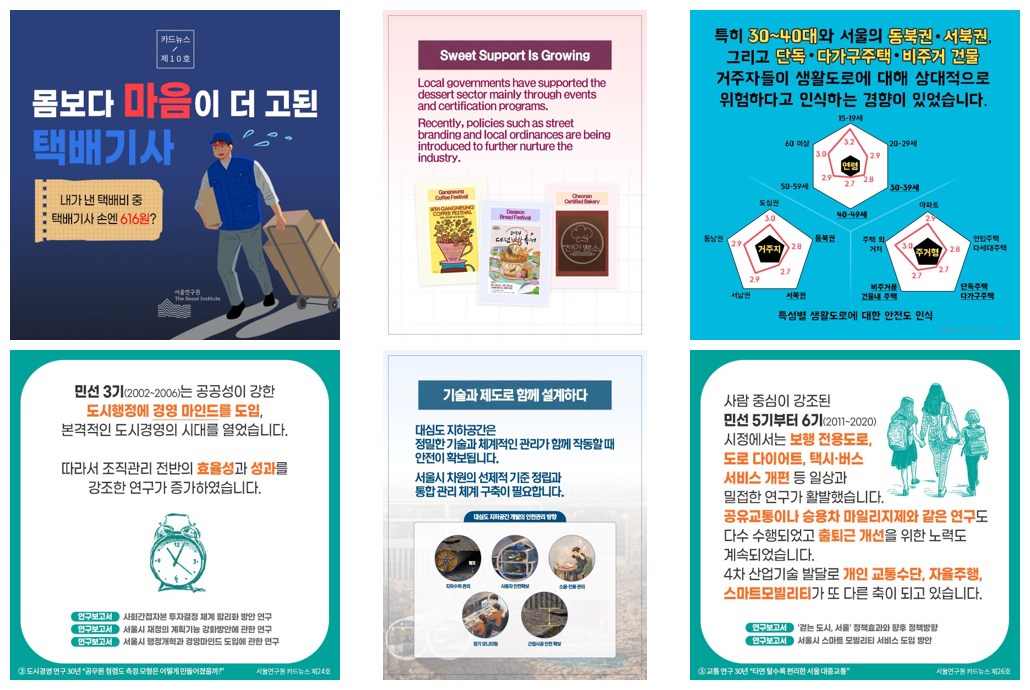
\includegraphics[width=\linewidth]{fig_dataset.png}
  \caption{Representative pages from the 687-image, 66-deck Korean card-news corpus.}
  \label{fig:dataset}
\end{figure}

\textbf{Automatic labeling.} Manual box annotation does not scale, so we generate
\emph{pseudo-labels}: EasyOCR~\cite{easyocr} is run at high recall
(\texttt{canvas\_size}=2560, \texttt{mag\_ratio}=2.0, \texttt{low\_text}=0.3) to
recover small body text; each text line is typed as \emph{title} when its height
exceeds 4.5\% of the image height, else \emph{body}. Because layout generation
needs element \emph{regions} rather than individual lines, we merge neighboring
lines of the same class into \textbf{blocks} via a union-find over boxes expanded
by a fraction of their height. This yields 284 title and 641 body boxes on the
seed set; \texttt{logo}/\texttt{underlay} remain for manual annotation.

\section{Method}
\label{sec:method}
Figure~\ref{fig:pipeline} summarizes the system: collect $\rightarrow$ detect
$\rightarrow$ \{template engine $\mid$ DS-GAN\} $\rightarrow$ render.

\begin{figure}[t]
  \centering
  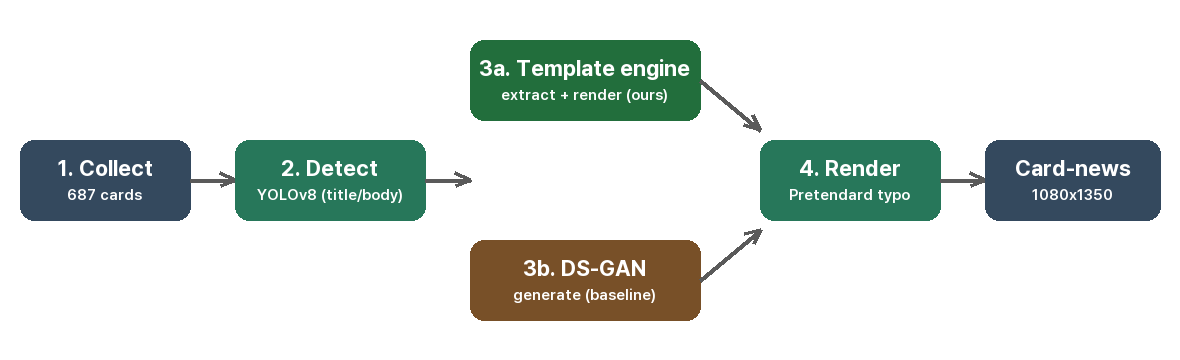
\includegraphics[width=\linewidth]{fig_pipeline.png}
  \caption{System overview. A shared detector feeds two generation routes; the
  template engine (3a) is our deployed path, DS-GAN (3b) is the research baseline.}
  \label{fig:pipeline}
\end{figure}

\subsection{Element detection}
We fine-tune YOLOv8-nano (and -small) from COCO weights on the pseudo-labels.
Horizontal flipping is disabled (\texttt{fliplr}=0) because it mirrors Hangul; we
use a card-tuned augmentation set (mild mosaic, HSV jitter, small scale/translate,
random erasing). The detector both (a) supplies masks for inpainting and the
\texttt{train\_csv} used by DS-GAN, and (b) \emph{extracts the layout templates}
described next.

\subsection{Layout generation: two routes}
\textbf{(3b) DS-GAN baseline.} Following PosterLayout~\cite{posterlayout2023}, we
construct the required \texttt{Dataset/} (inpainted posters, dual saliency maps,
\texttt{train\_csv} of normalized element boxes) using U$^2$-Net/BASNet saliency
and LaMa inpainting, and fine-tune DS-GAN to generate (class, box) layouts on
clean Korean backgrounds. While the model produces plausible boxes, its
\emph{rendered} output is not deployable: it cannot place legible Korean
glyphs and layout stability varies run-to-run.

\textbf{(3a) Detection-driven template engine (ours).} We instead \emph{copy and
re-render} real layouts. The detector localizes title/body blocks on a reference
card; classical inpainting (or LaMa) removes the original text; new content is
typeset back into the same block geometry with the Pretendard~\cite{pretendard}
typeface. We additionally maintain a small library of layout archetypes
(editorial, centered, bottom-panel, cover) distilled from the corpus, and a
saliency-aware placement step that selects the calmest image band (lowest mean
gradient magnitude) for text and applies a luminance-adaptive scrim so the result
is legible over \emph{any} background.

\subsection{Rendering}
Cards are composited at $1080\times1350$ (Instagram 4:5). Text color is chosen
from the background luminance under each block (white on dark, near-black on
light), font size is auto-fit per box, and a soft rounded scrim guarantees
contrast and covers residual texture. Typography uses Pretendard Bold for titles
and Regular for body, with a fixed spacing system and accent rules.

\section{Sequential Analysis of Decks}
\label{sec:timeseries}
A card-news deck is an ordered sequence of pages; we treat the page index as a
discrete time axis and ask how layout/visual structure evolves along it. Over the
66 decks ($\geq 4$ pages each) we compute, per page, four cv2 features---Canny
\emph{edge density} (text/graphic density), \emph{brightness}, Hasler--S\"usstrunk
\emph{colorfulness}~\cite{hasler2003colorfulness}, and HSV \emph{saturation}---and
average them into ten relative-position bins ($0$=cover, $1$=last).

Figure~\ref{fig:timeseries} shows a consistent \textbf{cover-vs-interior}
pattern: covers are notably \emph{darker} (brightness $0.62$ vs.\ $\approx0.71$
for interiors), more \emph{saturated} ($0.33$ vs.\ $\approx0.27$) and more
\emph{colorful}, and have the \emph{lowest edge density} ($0.097$). Interior pages
are brighter and denser (more text), and the final page partly reverts toward the
cover's saturated tone. This quantifies a design convention---an eye-catching,
high-chroma cover followed by readable content pages---and motivates
\emph{position-conditioned} templates (Sec.~\ref{sec:method}): the engine selects
a cover archetype for page~1 and content archetypes thereafter.

\begin{figure}[t]
  \centering
  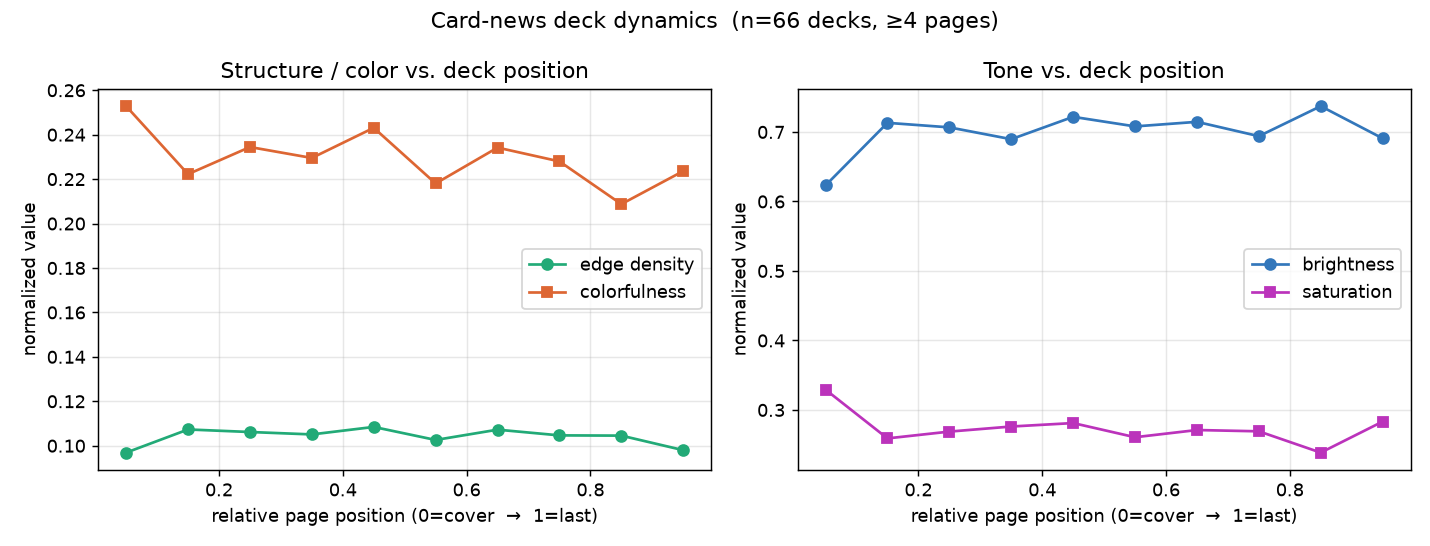
\includegraphics[width=\linewidth]{fig_timeseries.png}
  \caption{Deck dynamics across relative page position (66 decks). Covers are
  darker, more saturated/colorful and less edge-dense than interior pages.}
  \label{fig:timeseries}
\end{figure}

\section{Experiments}
\label{sec:exp}
\textbf{Setup.} YOLOv8 fine-tuning, $640$\,px, 150--300 epochs, batch tuned to GPU;
metrics are box mAP. The seed split is 93 train / 16 val. Cloud training uses an
RTX 4090; development/inference run on an RTX 3050.

\subsection{Detector ablation}
Table~\ref{tab:ablation} and Figure~\ref{fig:ablation} report the ablation.
Transfer learning is the dominant factor (scratch $0.502$ vs.\ baseline $0.662$).
A card-tuned augmentation and a longer schedule give the best nano model
(\texttt{long300\_card}: mAP@50--95 $=0.718$, mAP@50 $=0.854$); YOLOv8-small is
competitive ($0.705$). Seed repeats vary by $<0.02$ mAP, indicating stable
ranking. Qualitative detections are shown in Figure~\ref{fig:detector}.

\begin{table}[t]
\centering
\small
\begin{tabular}{lcc}
\toprule
Configuration & mAP@50--95 & mAP@50 \\
\midrule
scratch (no pretrain)        & 0.502 & 0.736 \\
baseline (n, freeze 10)      & 0.662 & 0.844 \\
freeze 0                     & 0.671 & 0.851 \\
aug: heavy                   & 0.644 & 0.838 \\
aug: card-tuned              & 0.696 & 0.838 \\
img 768                      & 0.680 & 0.841 \\
YOLOv8-s (freeze 10)         & 0.705 & 0.852 \\
\textbf{long300 + card aug (best)} & \textbf{0.718} & \textbf{0.854} \\
\bottomrule
\end{tabular}
\caption{Detector ablation on the 109-image seed set (pseudo-labels).}
\label{tab:ablation}
\end{table}

\begin{figure}[t]
  \centering
  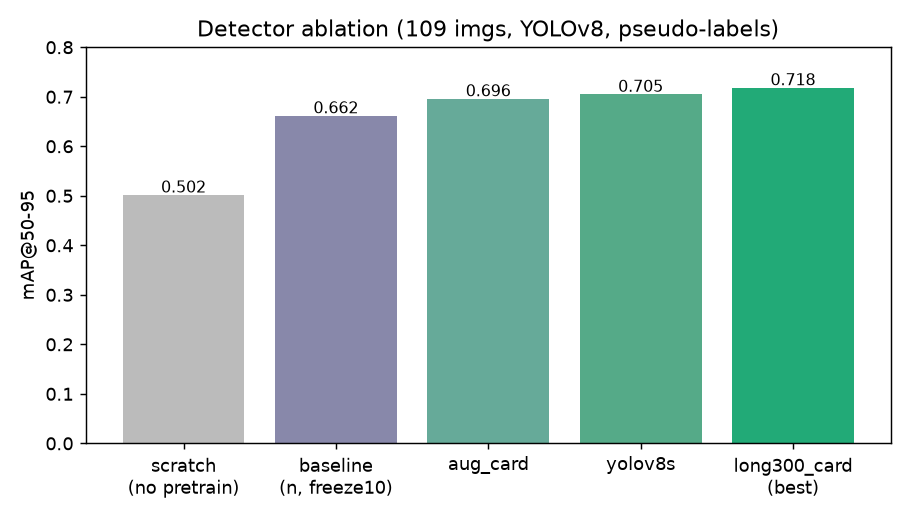
\includegraphics[width=\linewidth]{fig_ablation.png}
  \caption{Key ablation results (box mAP@50--95). Transfer learning and a
  card-tuned, longer schedule drive the gains.}
  \label{fig:ablation}
\end{figure}

\begin{figure}[t]
  \centering
  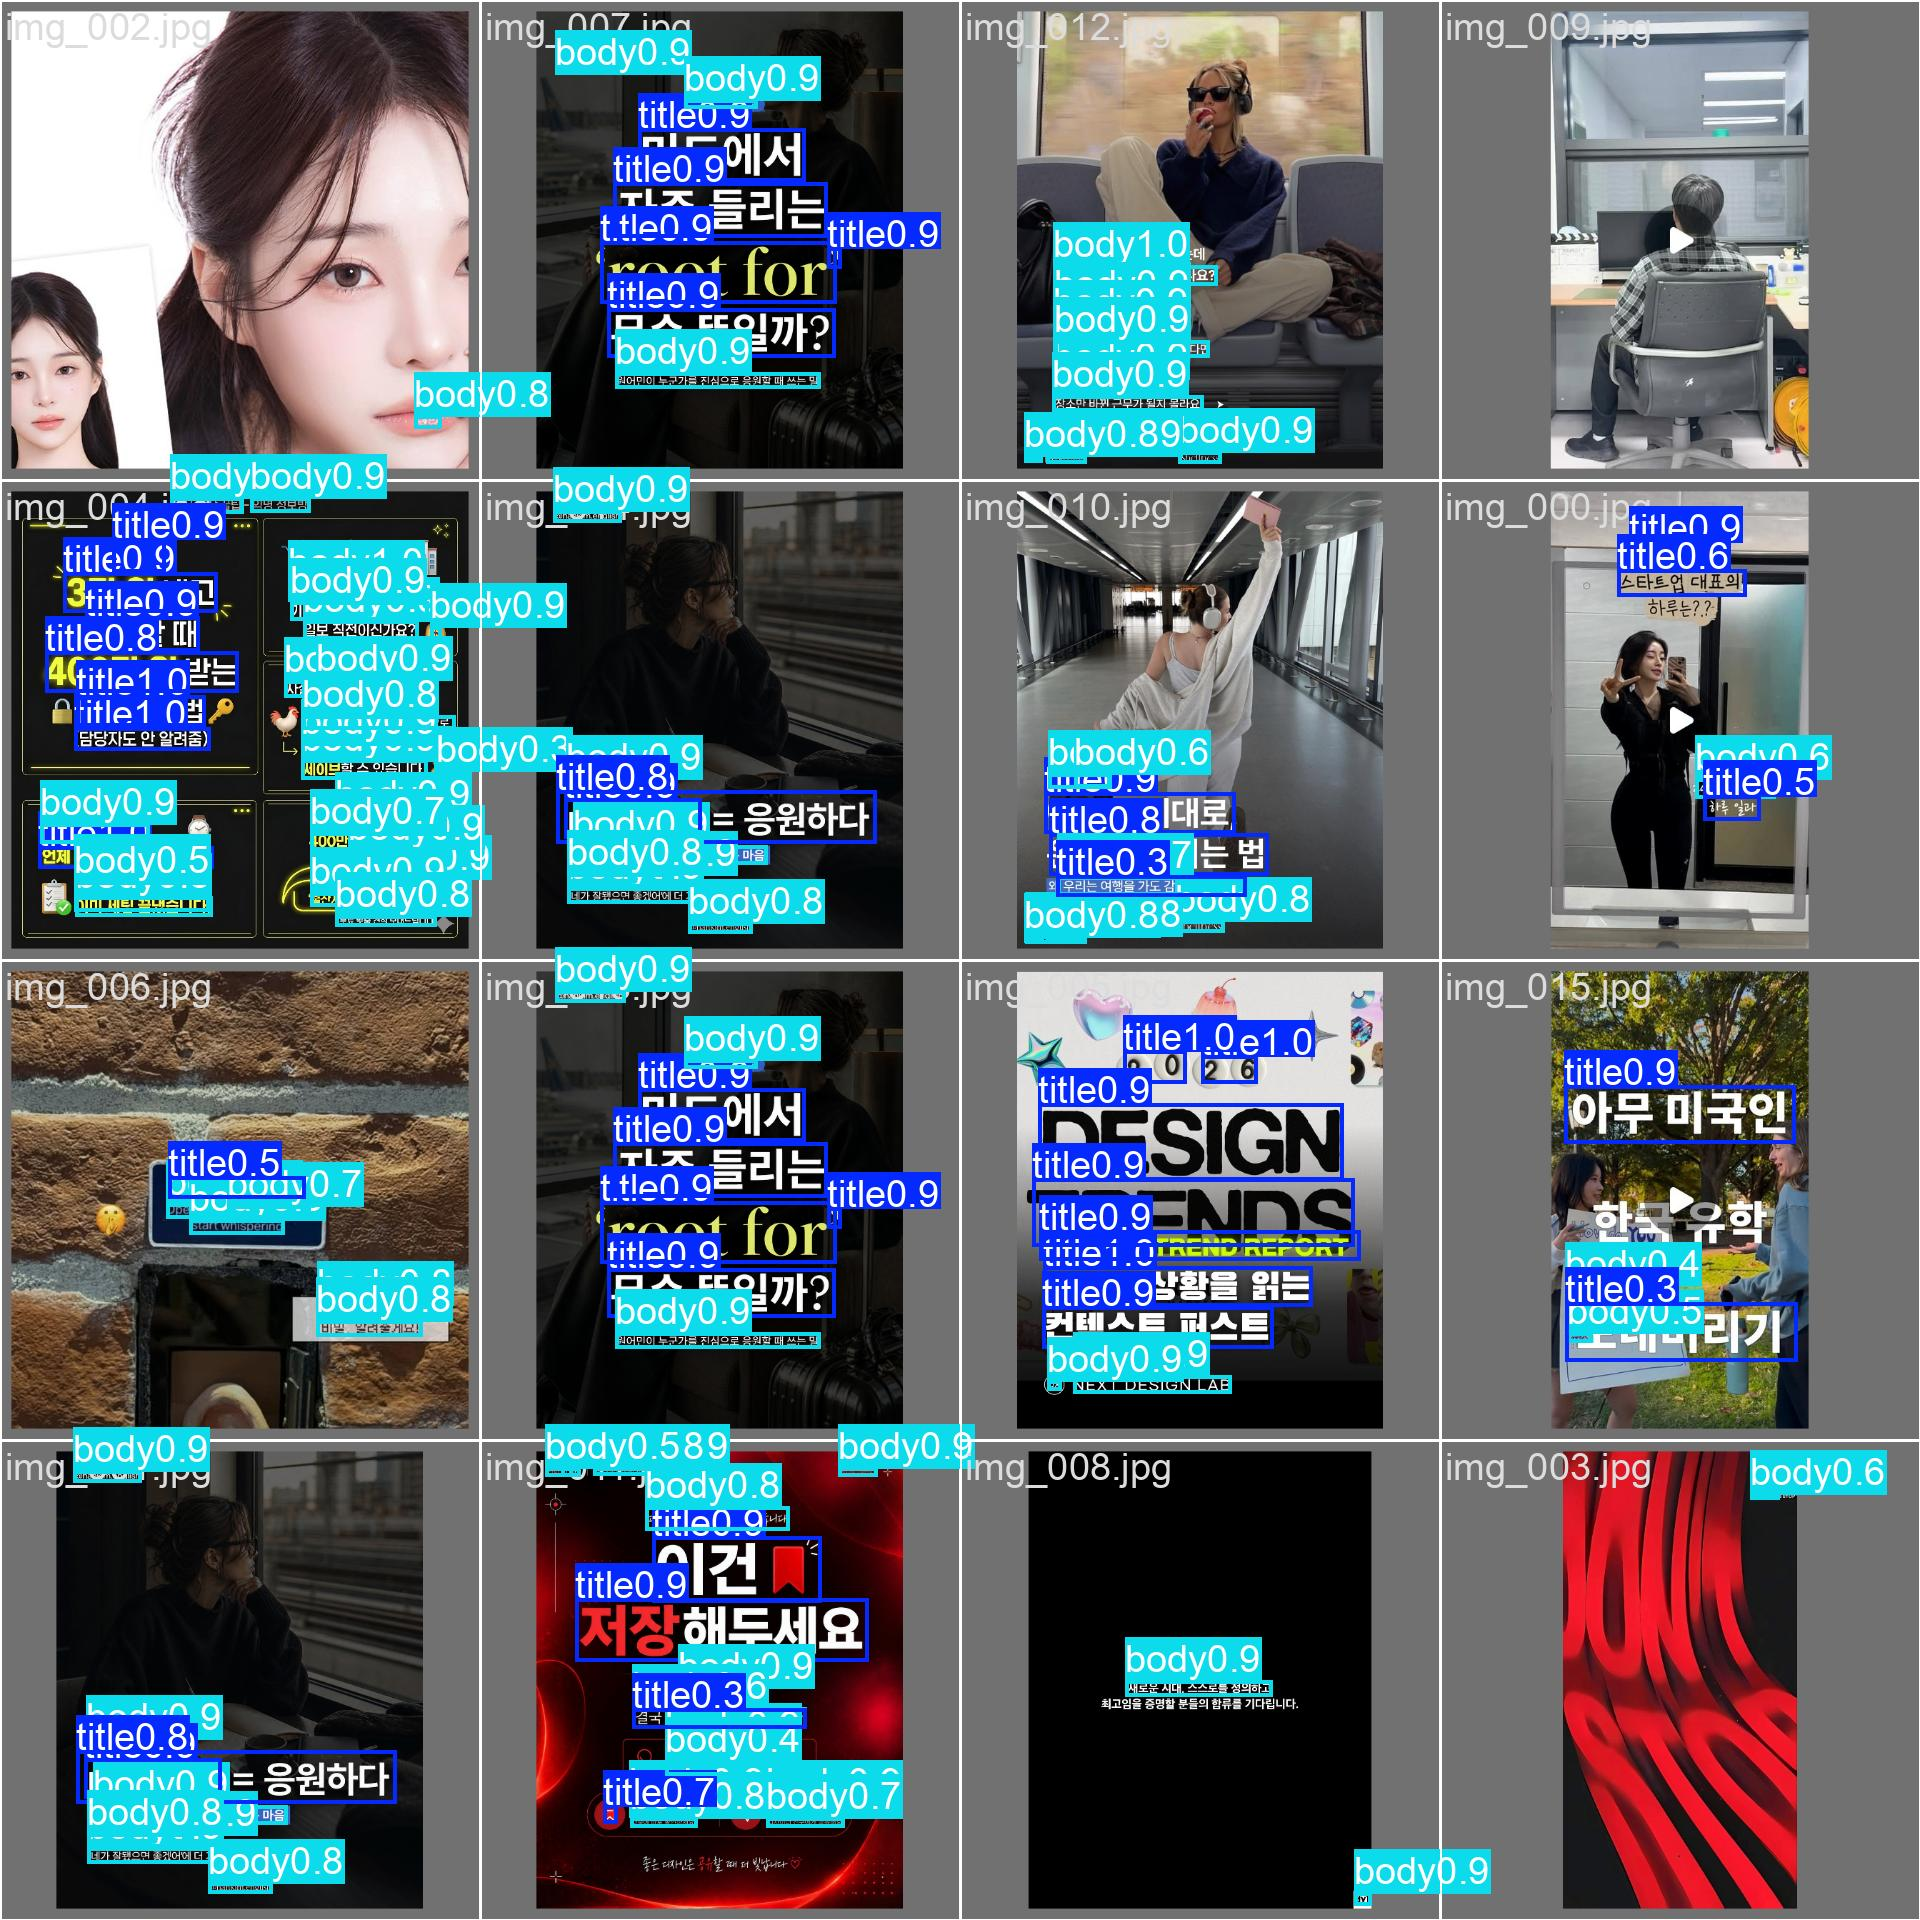
\includegraphics[width=\linewidth]{fig_detector_pred.jpg}
  \caption{Detector predictions on held-out validation cards (title/body).}
  \label{fig:detector}
\end{figure}

\textbf{Robustness (5-fold CV).} Five-fold cross-validation of the baseline gives
mAP@50--95 $=0.611\pm0.049$, confirming the small-data result is not split-specific.

\textbf{Data scale (109 vs.\ 687).} To measure the effect of the 578 new images we
adopt a \emph{leak-free} protocol: a common test set (15\% of the new images) is
held out and never trained on, and the best recipe is trained on (i) the 109 seed
images and (ii) the full 687, with both evaluated on the identical test set. The
tooling is released; cloud training of this comparison is in progress and we
report it as a protocol rather than a completed result, to avoid drawing
conclusions from unfinished runs.

\subsection{Generation quality}
Figure~\ref{fig:results} shows template-engine outputs and a copy-and-re-render
example (original $\rightarrow$ cleaned background $\rightarrow$ recomposed). The
template engine yields legible, consistently designed Korean cards at
$1080\times1350$, whereas the DS-GAN route produces usable \emph{boxes} but not
deployable rendered text. For a production card-news service we therefore adopt
the template engine and retain DS-GAN as a research comparison.

\begin{figure}[t]
  \centering
  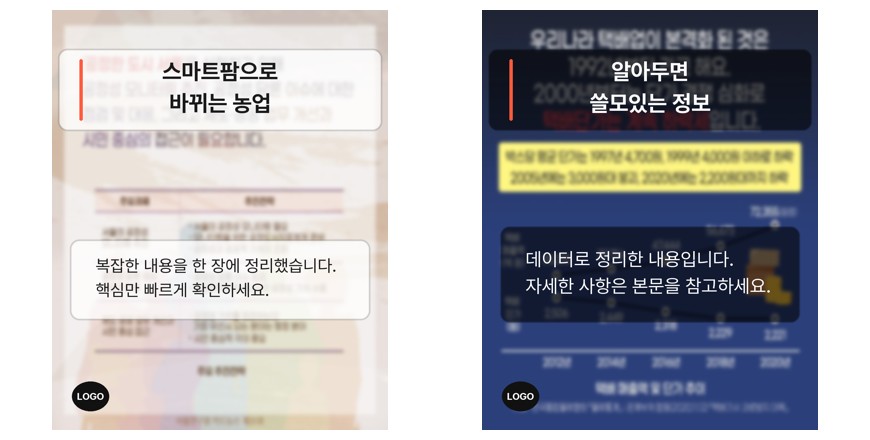
\includegraphics[width=\linewidth]{fig_results_template.png}\\[3pt]
  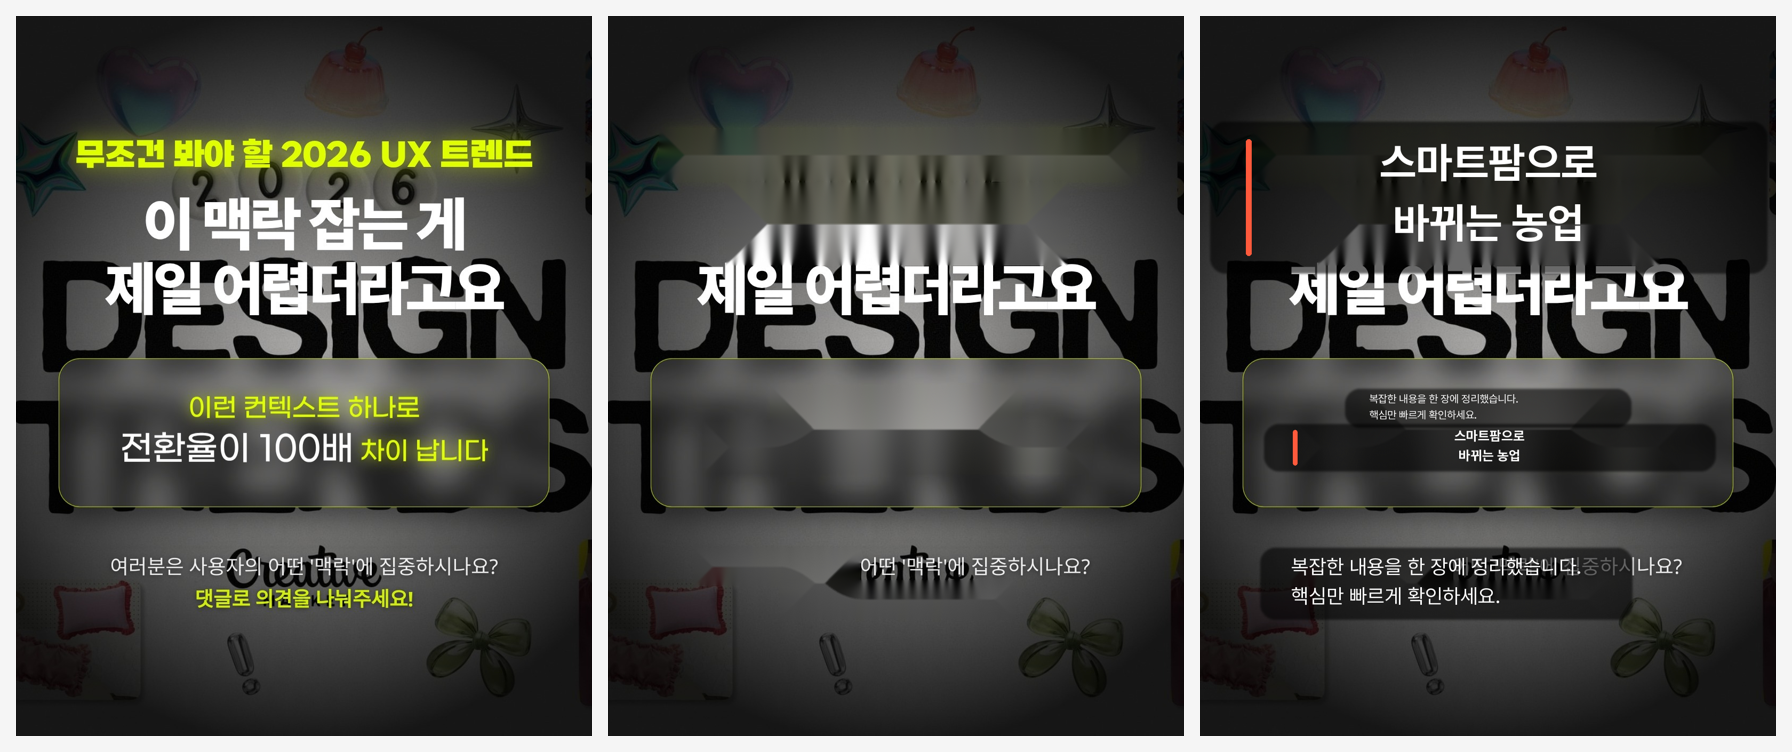
\includegraphics[width=\linewidth]{fig_results_copy.png}
  \caption{Top: template-engine cards (high-res, Pretendard, adaptive color).
  Bottom: layout copy---\emph{original $\mid$ inpainted background $\mid$
  recomposed} with new text in the analyzed layout.}
  \label{fig:results}
\end{figure}

\section{Discussion and Limitations}
Pseudo-labels cap detector quality: EasyOCR misses very small or stylized text,
so label recall---not data volume---is the binding constraint, addressed here by
high-recall OCR settings and block merging, and in future by CRAFT~\cite{craft2019}
or manual \texttt{logo}/\texttt{underlay} annotation. The DS-GAN route is limited
by Korean glyph rendering and small-data instability. The sequential analysis uses
low-level proxies; detector-derived element statistics per page are a natural
extension.

\section{Conclusion}
We presented a reproducible pipeline for Korean card-news layout: a curated
687-image, 66-deck corpus with automatic block labels, a fine-tuned YOLOv8
detector (mAP@50--95 $=0.718$), two generation routes whose comparison favors a
detection-driven template engine for deployment, and a time-series analysis that
reveals a quantifiable cover-vs-interior design convention. The artifacts provide
a basis for a practical Korean card-news generation service.

{\small
\bibliographystyle{ieeetr}
\bibliography{refs}
}

\end{document}
